\chapter{Backgroud}

 As the ORBM builds on the previous work of Restricted Boltzmann Machines and Sigmoid Belief networks, the concepts and previous work in source separation, generative models as well as background on RBMs and Sigmoid Belief Networks need to be introduced.

\section{Source Separation}

\subsection{An example, the cocktail party problem}
A famous example that illustrates the idea of source separation is the cocktail party problem. At a cocktail party many conversations are taking part at the same time, creating noise, a composition of all the conversations. Despite this, a partygoer is able to separate their conversation from cacophany, separating the sources.

The applications of source separation are far wider than talkative partygoers. In the field of signal processing
\todo%

\section{Generative Models}

Generative models are a powerful way to model data.
\todo%
(TODO-GRAB-THOSE-GENERATIVE-MODEL-USES-CITATIONS) Basically justify generative models.

The ORBM proposed in this project aims to represent data generated by two indepedanlty acting causes and does so by combining two existing generative models, the Restricted Boltzmann Machine, and the Sigmoid Belief Network.

\subsection{Modeling building blocks, observable and hidden variables}

Generative models are comprised of variables, often referred to as units. Some of these variables are observed, that is their state is known. These are often referred to as the `visible` units and are used to represent the training data. For example in the image domain, the visible units correspond to the pixels of the image.

The variables that are not observed, are latent variables, often referred to as `hidden units` as they are not observed.

Connections between units are used to encode relationships between the variables, where the relationship may be causal, such as in a Sigmoid Belief network or an encoding/representation in the Restricted Boltzmann Machine.


\subsection{PGMs as a tool reasoning about generative models}
\todo%
Probalistic Graphical Models or PGMs for short, are an expressive way to represent a collection of related, stochastic variables. If the graph is directed then the edges represent causation, this is also referred to a Bayesian network. Conversely, if the graph was undirected then edges represent a dependancy or mapping. Throughout this report, RBMs, Sigmoid Belief Networks and the proposed ORBM will be shown in this format.

Figure \ref{F:PGM-example} shows an abstract example of a directed PGM, where B is the underlying cause of A, we cannot observe B directly, instead it's state is represented as a `belief` or a probability of being in a given state.

\begin{figure}[h]
\begin{center}
  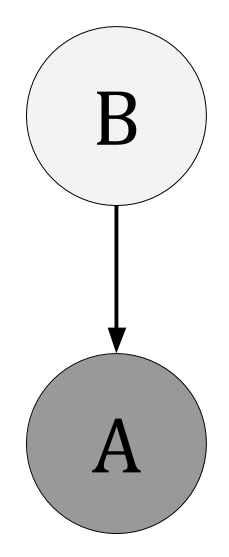
\includegraphics[width = 0.1\textwidth]{Assets/PGM_Example_1.png}
\caption{An example PGM, showing an observed variable `A` and it's hidden cause `B`.}
\label{F:PGM-example}
\end{center}
\end{figure}

\section{Sampling and inverting the model}
Sampling is the process of drawing samples from a distribution. It is used when the distrubtion we want samples from is intractable to calculate analytically. Sampling is required to train generative models, as often the gradient to be climbed/descended involves calculating a probability in the
generative model.
\todo%
\begin{itemize}
  \item Inference is the process of given reasoning about what we do not know given that of which we do know.
  \item In a Generative Model this amounts to the Posterior
\end{itemize}

\subsection{Gibbs sampling, a subset of Markov Chain Monte Carlo}

\begin{itemize}
  \item The importance of Markov Chains and mixing time are crutial in this project
\end{itemize}

Gibbs sampling is a special case of Markov Chain Monte Carlo, a technique for drawing sampling from a complex distribution. The probability mass (the joint distribution) of a generative model is a common use case for Gibbs sampling, and is used for performing inference in the RBMs, Sigmoid Belief Networks and in the ORBM. Being a specific case of Markov Chain Monte Carlo (refferred to as MCMC).

\subsubsection{Mixing Time}
MCMC methods require a `mixing` phase to ensure convergence, that is that the sample is being drawn from a representative part of the desired distribution. This is part of the trade off the ORBM attempts to make, as a mixing time is introduced that is not present in the RBM.

\subsection{Reconstructions, visualising what the model has learnt}

Generative Models can create an internal representation given an input. They can also generate a faux input given an internal representation. Performing one Gibbs iteration, that is sampling from the hidden units given an input $ P(\tilde{h}|\tilde{v}) $ and then taking the generated hidden state and generating a faux input. The model tries to reconstruct the input.

\subsubsection{Fanstasies of the model}
\todo%
In the same way that a generative model uses reconstructions to try and recreate the  supplied input based purely on how it's represented that input, performing many, many (greater than 100) Gibbs iterations with no input pattern clamped allows the reconstructions to explore the probability mass that the model has built up during training. Sampling from these wanderings creates what are refferred to as `fantasies` or `dreams`. These give a sense of what the model has learnt, and can act a smoke test for if the model has actually capture anything.
(TODO-CITE-PAPER-WITH-MNIST-DREAM-EVALUATION, they were crappy).
